\chapter{Specifikacija programske potpore}

    \section{Funkcionalni zahtjevi}

    \noindent \textbf{Dionici:}
		\begin{packed_enum}
			\item Vlasnik obrta (naručitelj)
			\item Korisnici				
            \item Razvojni tim
		\end{packed_enum}
			
    \noindent \textbf{Aktori i njihovi funkcionalni zahtjevi:}
		\begin{packed_enum}
			\item  \underbar{Vlasnik obrta (inicijator) može:}
			\begin{packed_enum}
				\item dodati ili obrisati obrt
                \item dodati, izbrisati ili promijeniti
				\begin{packed_enum}
					\item  naziv i opis obrta
					\item  kategoriju lokacije 
				\end{packed_enum}
                \item  pregledavati i odgovarati na recenzije korisnika
                \item  pretplatom na aplikaciju osigurati neke dodatne pogodnosti poput reklame
			\end{packed_enum}
                
            \item  \underbar{Neregistrirani korisnik (inicijator) može:}
			\begin{packed_enum}
				\item pregledati na karti prikladno ili neprikladno označene lokacije za       pse, te plaćene lokacije koje su dodatno istaknute
                \item pretraživati specifičnu lokaciju ili odabrati kategoriju čiji se markeri onda prikazuju
                \item  odabirom markirane lokacije saznati više informacija o odabranom položaju (ime lokacije, ocjenu i  kategorija) ili u slučaju obrta (naziv obrta, ocjenu, tip obrta, opis obrta i kontakt)
                \item  se registrirati u sustav stvaranjem novog korisničkog računa
			\end{packed_enum}
            \eject

            \item  \underbar{Registrirani korisnik (inicijator) može:}
			\begin{packed_enum}
				\item označavati novu lokaciju što uključuje unos imena lokacije te odabir njene kategorije
                \item potvrditi ili negirati oznaku neke već postojeće lokacije
                \item pregledavati i mijenjati osobne podatke
                \item izbrisati svoj korisnički račun
                \item pisati recenziju i dati ocjenu  
			\end{packed_enum}
				
            \item  \underbar{Baza podataka (sudionik) može:}
			\begin{packed_enum}
				\item pohranjuje sve podatke o 
                \begin{packed_enum}
				    \item  korisnicima i njihovim ovlastima
				    \item  obrtima i njihovoj kategoriji
				\end{packed_enum}
			\end{packed_enum}
        \end{packed_enum}
	\eject 
    
    \subsection{Obrasci uporabe}
		\textbf{Opis obrazaca uporabe}
			
	    	\noindent\underbar{\textbf{UC1: Registracija korisnika}}
				\begin{itemize}
					\item \textbf{Glavni sudionik: } Korisnik 
					\item \textbf{Cilj: }Omogućiti korisniku prijavu u sustav, čime će korisnik ostvariti pravo na  korištenje više funkcijonalnosti aplikacije 
					\item \textbf{Sudionici: } Baza podataka 
					\item \textbf{Preduvjet: } - 
					\item \textbf{Opis osnovnog tijeka: }
					\begin{enumerate}
						\item Korisnik odabire opciju za registraciju
						\item Korisnik u registracijskom sučelju popunjava formu sa svojim podacima
						\item Korisnik dobiva e-mail na unesenu adresu u kojem potvrđuje svoju registraciju
					\end{enumerate}
					\item \textbf{Opis mogućih odstupanja:}
					\begin{itemize}
						\item Korisnik nije unio sve obavezne podatke
						\item Odabir već zauzetog korisničkog imena i/ili e-maila
						\item Unos podatka u nedozvoljenom formatu
					\end{itemize}
				\end{itemize}
					
			\noindent\underbar{\textbf{UC2: Prijava}}
				\begin{itemize}
					\item \textbf{Glavni sudionik: } Korisnik, vlasnik obrta 
					\item \textbf{Cilj: }Dobiti pristup korisničkom sučelju s dodatnim funkcionalnostima
					\item \textbf{Sudionici: } Baza podataka 
					\item \textbf{Preduvjet: } Uspješna registracija 
					\item \textbf{Opis osnovnog tijeka: }
					\begin{enumerate}
						\item Unos korisničkog imena i lozinke u formu za prijavu
						\item Potvrda o ispravnosti unešenih podataka
						\item Redirekcija na korisničko sučelje aplikacije
					\end{enumerate}
					\item \textbf{Opis mogućih odstupanja:}
					\begin{itemize}
						\item Pogrešno korisničko ime i/ili lozinka
					\end{itemize}
				\end{itemize}
					
			\noindent\underbar{\textbf{UC3: Pregled osobnih podataka}}
				\begin{itemize}
					\item \textbf{Glavni sudionik: } Korisnik, vlasnik obrta 
					\item \textbf{Cilj: }Omogućiti pregled osobnih podataka 
					\item \textbf{Sudionici: } Baza podataka 
					\item \textbf{Preduvjet: } Korisnik je prijavljen 
					\item \textbf{Opis osnovnog tijeka: }
					\begin{enumerate}
						\item Korisnik odabire opciju za prikaz osobnih podataka
						\item Prikaz osobnih podataka korisnika
					\end{enumerate}
				\end{itemize}
						
			\noindent\underbar{\textbf{UC4: Promjena osobnih podataka korisnika}}
				\begin{itemize}
					\item \textbf{Glavni sudionik: } Korisnik, vlasnik obrta 
					\item \textbf{Cilj: }Omogućiti promjenu korisničkog imena i/ili lozinke korisničkog računa 
					\item \textbf{Sudionici: } Baza podataka 
					\item \textbf{Preduvjet: } Korisnik je prijavljen 
					\item \textbf{Opis osnovnog tijeka: }
					\begin{enumerate}
						\item Korisnik odabire opciju za promjenom osobnih podataka
						\item Korisnik unosi nove osobne podatke i sprema promjene
						\item Promjene se spremaju u bazu podataka
					\end{enumerate}
					\item \textbf{Opis mogućih odstupanja:}
					\begin{itemize}
						\item Novo korisničko ime je zauzeto
					\end{itemize}
				\end{itemize}
					
			\noindent\underbar{\textbf{UC5: Brisanje korisničkog računa}}
				\begin{itemize}
					\item \textbf{Glavni sudionik: } Korisnik
					\item \textbf{Cilj: }Korisnik briše svoj korisnički račun
					\item \textbf{Sudionici: } Baza podataka 
					\item \textbf{Preduvjet: } Korisnik je prijavljen 
					\item \textbf{Opis osnovnog tijeka: }
					\begin{enumerate}
						\item Korisnik odabire opciju za brisanje svog korisničkog računa
						\item Odjava iz aplikacije
						\item Korisnički račun se briše iz baze podataka
						\item Redirekcija na naslovnu stranicu
					\end{enumerate}
				\end{itemize}
					
			\noindent\underbar{\textbf{UC6: Promjena podataka obrta}}
				\begin{itemize}
					\item \textbf{Glavni sudionik: } Vlasnik obrta 
					\item \textbf{Cilj: }Omogućiti vlasnicima obrta promjenu podataka o obrtima
					\item \textbf{Sudionici: } Baza podataka 
					\item \textbf{Preduvjet: } Vlasnik obrta je prijavljen
					\item \textbf{Opis osnovnog tijeka: }
					\begin{enumerate}
						\item Vlasnik obrta odabire opciju za promjenu podataka obrta
						\item Vlasnik mijenja ime, opis, kategoriju, OIB, kontakt broj i/ili neki drugi podatak
						\item Vlasnik sprema promjene
						\item Promjene se spremaju u bazu podataka
					\end{enumerate}
				\end{itemize}
					
			\noindent\underbar{\textbf{UC7: Brisanje računa vlasnika obrta}}
				\begin{itemize}
					\item \textbf{Glavni sudionik: } Vlasnik obrta 
					\item \textbf{Cilj: }Omogućiti vlasniku obrta brisanje računa
					\item \textbf{Sudionici: } Baza podataka 
					\item \textbf{Preduvjet: } Vlasnik obrta je prijavljen
					\item \textbf{Opis osnovnog tijeka: }
					\begin{enumerate}
						\item Vlasnik obrta odabire opciju za brisanje računa
						\item Odjava iz aplikacije
						\item Račun vlasnika obrta se briše iz baze podataka
                        \item Redirekcija na naslovnu stranicu
					\end{enumerate}
				\end{itemize}
					
			\noindent\underbar{\textbf{UC8: Pregled podataka lokacije}}
				\begin{itemize}
					\item \textbf{Glavni sudionik: } Korisnik, vlasnik obrta 
					\item \textbf{Cilj: }Pregled podataka bilo koje unesene lokacije
					\item \textbf{Sudionici: } Baza podataka 
					\item \textbf{Preduvjet: } -
					\item \textbf{Opis osnovnog tijeka: }
					\begin{enumerate}
						\item Učitava se karta sa unesenim lokacijama
						\item Klikom na pojedinu lokaciju prikazuju se njeni podaci
					\end{enumerate}
				\end{itemize}
					
			\noindent\underbar{\textbf{UC9: Potvrđivanje ili negiranje oznake postojeće lokacije}}
				\begin{itemize}
					\item \textbf{Glavni sudionik: } Korisnik, vlasnik obrta 
					\item \textbf{Cilj: }Omogućiti prijavljenim korisnicima da potvrde ili negiraju oznaku postojeće lokacije
					\item \textbf{Sudionici: } Baza podataka 
					\item \textbf{Preduvjet: } Korisnik ili vlasnik obrta su prijavljeni
					\item \textbf{Opis osnovnog tijeka: }
					\begin{enumerate}
						\item Kod prikaza informacija pojedine lokacije, korisnik odabire opciju potvrđivanja ili negiranja lokacije
						\item Informacija se sprema u bazu podataka
					\end{enumerate}
				\end{itemize}
					
			\noindent\underbar{\textbf{UC10: Označavanje novih lokacija}}
				\begin{itemize}
					\item \textbf{Glavni sudionik: } Korisnik, vlasnik obrta 
					\item \textbf{Cilj: }Omogućiti unos neke lokacije koja je (ne)prikladna za pse
					\item \textbf{Sudionici: } Baza podataka 
					\item \textbf{Preduvjet: } Korisnik ili vlasnik obrta su prijavljeni
					\item \textbf{Opis osnovnog tijeka: }
					\begin{enumerate}
						\item Korisnik odabire opciju za označavanjem nove lokacije
						\item Korisnik unosi ime i kategoriju lokacije te je li ona prikladna za pse
						\item Podaci se spremaju u bazu podataka
					\end{enumerate}
				\end{itemize}
					
			\noindent\underbar{\textbf{UC11: Prikaz lokacija po odabranoj kategoriji}}
				\begin{itemize}
					\item \textbf{Glavni sudionik: } Korisnik, vlasnik obrta 
					\item \textbf{Cilj: }Omogućiti prikaz lokacija na karti po odabranoj kategoriji
					\item \textbf{Sudionici: } Baza podataka 
					\item \textbf{Preduvjet: } -
					\item \textbf{Opis osnovnog tijeka: }
					\begin{enumerate}
						\item Korisnik na karti odabire kategoriju po kojoj želi filtrirati lokacije
						\item Na karti se prikazuju samo lokacije sa odabranom kategorijom
					\end{enumerate}
				\end{itemize}		
				
			\noindent\underbar{\textbf{UC12: Registracija vlasnika obrta}}
				\begin{itemize}
					\item \textbf{Glavni sudionik: } Vlasnik obrta 
					\item \textbf{Cilj: }Omogućiti vlasniku obrta prijavu u sustav, čime će vlasnik obrta ostvariti pravo na korištenje više funkcijonalnosti aplikacije
					\item \textbf{Sudionici: } Baza podataka 
					\item \textbf{Preduvjet: } -
					\item \textbf{Opis osnovnog tijeka: }
					\begin{enumerate}
			    		\item Vlasnik obrta odabire opciju za registraciju
						\item Vlasnik obrta u registracijskom sučelju popunjava formu sa svojim podacima i podacima obrta
                        \item Vlasnik obrta na unesenu e-mail adresu dobiva potvrdu o uspješnoj registraciji i uspješnom plaćanju
					\end{enumerate}
                    \item \textbf{Opis mogućih odstupanja:}
					\begin{itemize}
						\item Vlasnik obrta nije unio sve obavezne podatke
						\item Odabir već zauzetog korisničkog imena i/ili e-maila
						\item Unos podatka u nedozvoljenom formatu
					\end{itemize}
				\end{itemize}

            \noindent\underbar{\textbf{UC13: Pisanje recenzija i davanje ocjena lokacijama i obrtima}}
				\begin{itemize}
					\item \textbf{Glavni sudionik: } Korisnik
					\item \textbf{Cilj: }Napisati recenziju i ocijeniti lokaciju ili obrt
					\item \textbf{Sudionici: } Baza podataka 
					\item \textbf{Preduvjet: } Korisnik je prijavljen
					\item \textbf{Opis osnovnog tijeka: }
					\begin{enumerate}
						\item Korisnik napiše recenziju i ocijeni lokaciju ili obrt
						\item Ocjena i recenzija se pohranjuju u bazu podataka i ažurira se prosječna ocjena lokacije ili obrta 
					\end{enumerate}
                    \item \textbf{Opis mogućih odstupanja:}
					\begin{itemize}
						\item Korisnik ne želi napisati osvrt
					\end{itemize}
				\end{itemize} 

            \noindent\underbar{\textbf{UC14: Pregled recenzija korisnika}}
			    \begin{itemize}
					\item \textbf{Glavni sudionik: } Vlasnik obrta
					\item \textbf{Cilj: }Pregledati recenzije korisnika za vlasnikov obrt 
					\item \textbf{Sudionici: } Baza podataka 
					\item \textbf{Preduvjet: } Vlasnik obrta je prijavljen
					\item \textbf{Opis osnovnog tijeka: }
					\begin{enumerate}
						\item Vlasnik odabire opciju “Pregledaj recenzije“
						\item Prikažu se sve dotadašnje recenzije i ocjene vlasnikovog obrta
					\end{enumerate}
				\end{itemize} 	
			
	\pagebreak
	\subsection*{Dijagrami obrazaca uporabe}
    	\begin{figure}[H]
            \centering                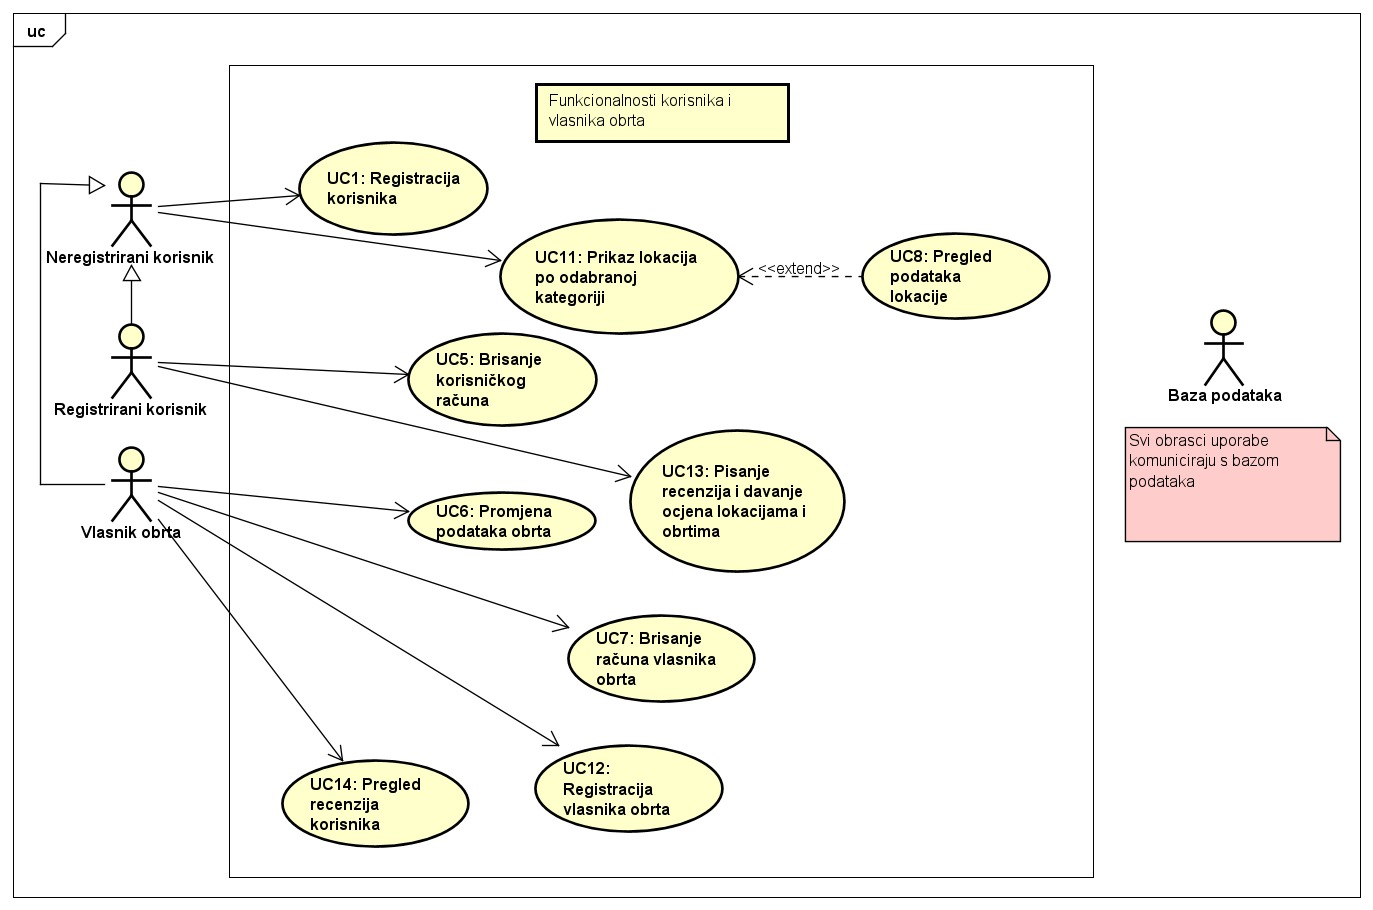
\includegraphics[width=\textwidth]{img/UseCaseDiagram1.png}
            \caption{Funkcionalnost korisnika i vlasnika obrta}
        \end{figure}
		\begin{figure}[H]
			\centering
			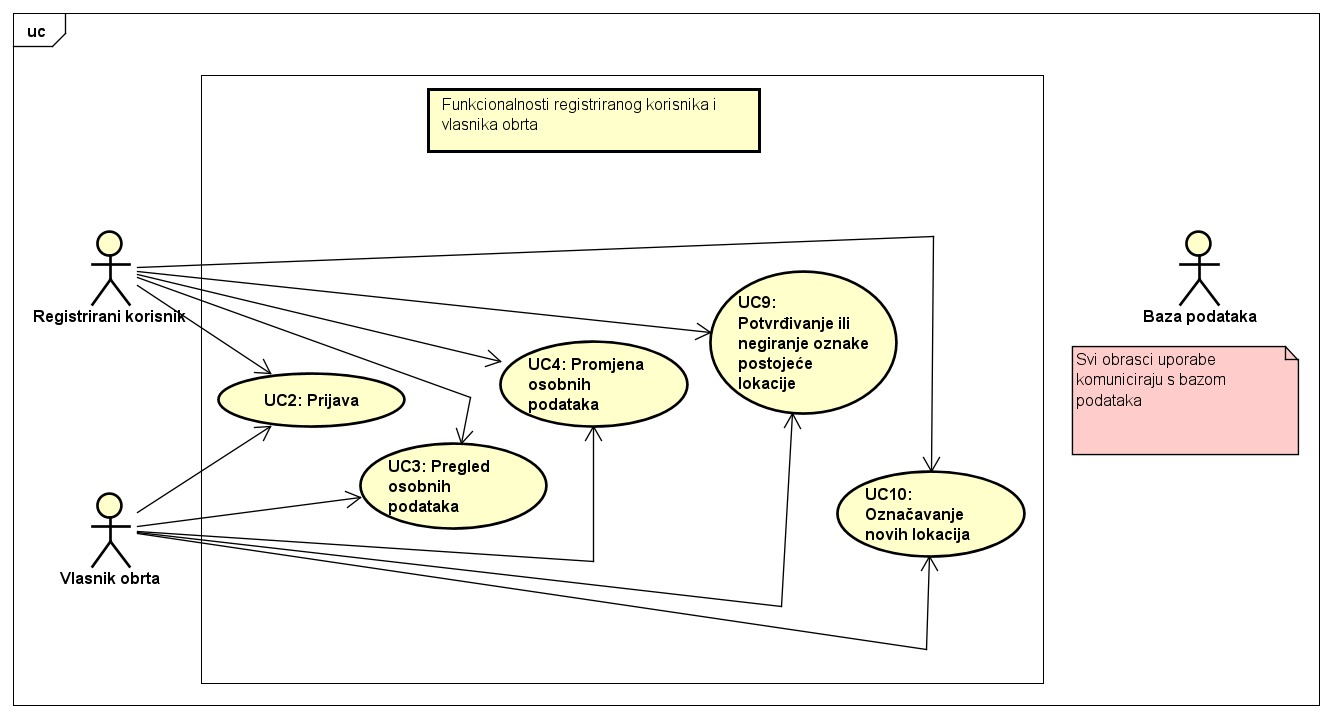
\includegraphics[width=\textwidth]{img/UseCaseDiagram2.png}
			\caption{Funkcionalnost registriranog korisnika i vlasnika obrta}
			    \end{figure}

    \subsection{Sekvencijski dijagrami}
		\textbf{Obrasci uporabe UC1 i UC12 - Registracija}
				
		Korisnik ili vlasnik obrta šalje zahtjev za registracijom koji za osnovne korisnike sadrži e-mail adresu, korisničko ime, lozinku, ime, prezime i opis. Zahtjev za registraciju vlasnika obrta sadrži e-mail adresu, lozinku te naziv, adresu, OIB, kontakt broj, djelatnost i kratki opis obrta. Web aplikacija validira ulazne podatke te se podaci spremaju u bazu podataka. Korisniku se nakon toga na navedenu e-mail adresu šalje link za verifikaciju računa.
			\begin{figure}[H]
				\centering
				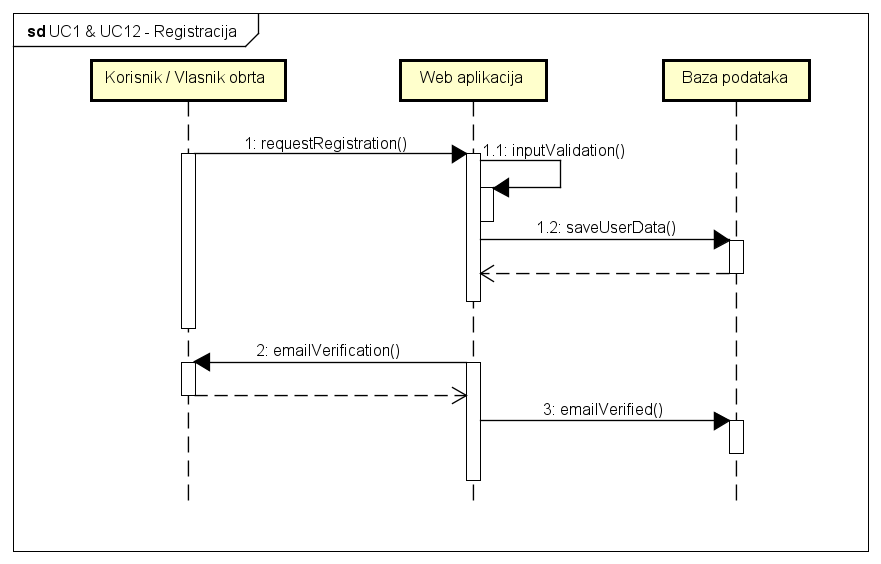
\includegraphics[width=\textwidth]{img/UC1&UC12-Registracija.png}
				\caption{Sekvencijski dijagram registracije korisnika ili vlasnika obrta}
			\end{figure}
			
			\pagebreak \noindent \textbf{Obrazac uporabe UC9 - Potvrđivanje ili negiranje oznake postojeće lokacije}
			
			Korisnik ili vlasnik obrta šalje zahtjev za učitavanjem karte na naslovnoj stranici, podaci se povlače iz baze podataka te se lokacije iscrtavaju na karti. Klikom na neku od lokacija korisniku se prikazuju osnovni podaci odabrane lokacije ili obrta. Ukoliko je korisnik(ili vlasnik obrta) prijavljen, on može potvrditi ili negirati postojanje označene lokacije, što će se zatim spremiti u bazu podataka.
			\begin{figure}[H]
				\centering
				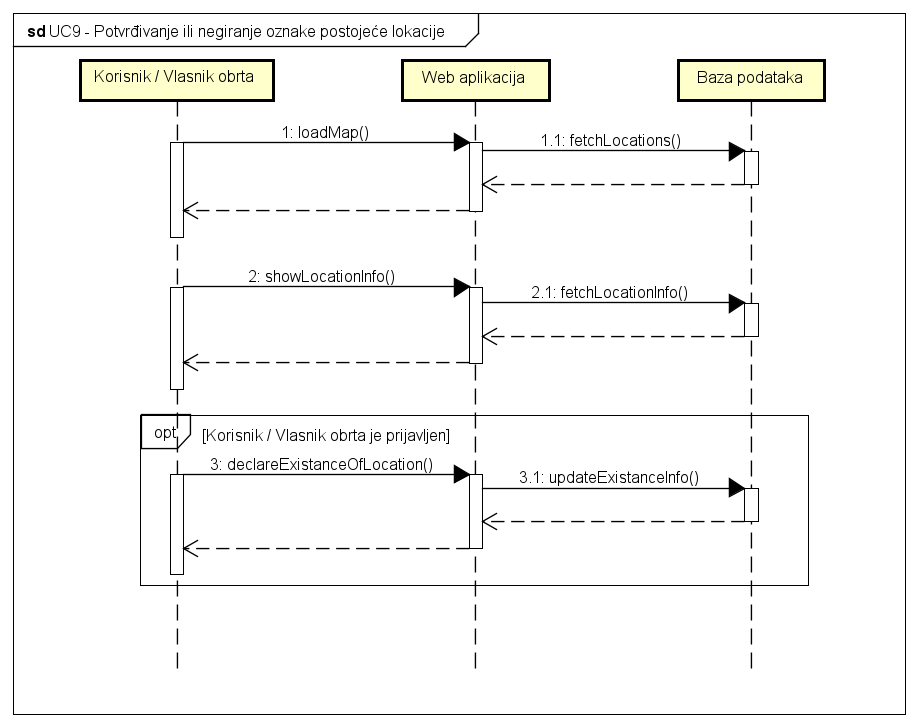
\includegraphics[width=\textwidth]{img/UC9-Potvrdivanje_ili_negiranje_oznake_postojece_lokacije.png}
				\caption{Sekvencijski dijagram potvrđivanja ili negiranja postojećih lokacija}
			\end{figure}
			
			\pagebreak \noindent \textbf{Obrazac uporabe UC10 - Označavanje novih lokacija}
			
			Korisnik prilikom učitavanja naslovne stranice šalje zahtjev za učitavanjem karte s lokacijama, uslijed čega web aplikacija povlači iz baze podataka potrebne podatke o lokacijama te ih iscrtava na karti. Registrirani i prijavljeni korisnik može označiti novu lokaciju na karti te za nju navesti ime lokacije, kategoriju te je li prikladna za pse. Uneseni podaci se spremaju u bazu podataka.
			\begin{figure}[H]
				\centering
				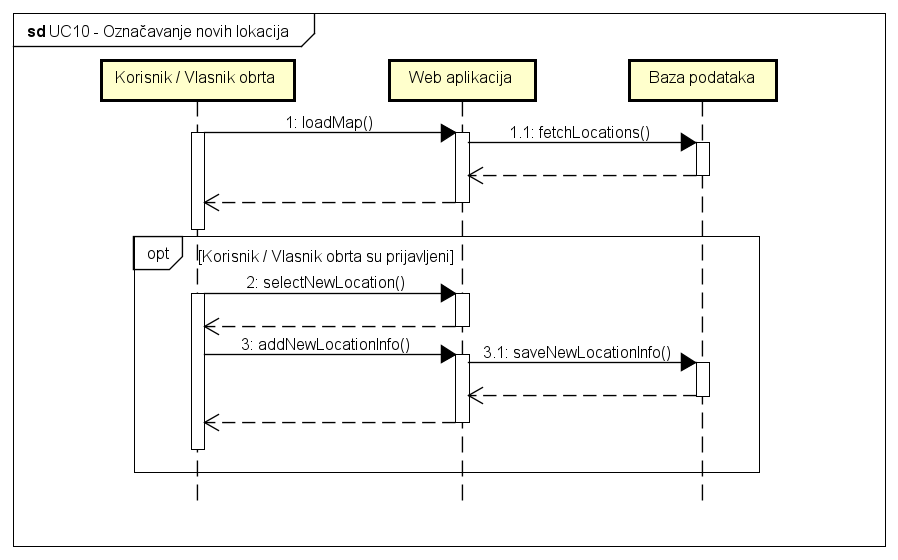
\includegraphics[width=\textwidth]{img/UC10-Oznacavanje_novih_lokacija.png}
				\caption{Sekvencijski dijagram označavanja novih lokacija}
			\end{figure}
			
			\pagebreak \noindent \textbf{Obrazac uporabe UC13 - Pisanje recenzija i ocjenjivanje lokacija}
			
			Korisniku se klikom na marker lokacije prikazuju osnovni podaci unesene lokacije ili obrta. Nadalje, korisnik može poslati zahtjev za recenzijama odabrane lokacije koje se zatim povlače iz baze podataka. Ukoliko je korisnik prijavljen, on može napisati vlastitu recenziju i/ili ocijeniti lokaciju s jednom do pet zvjezdica. Napisana recenzija i/ili odabrana ocjena se zatim spremaju u bazu podataka.
			
			\begin{figure}[H]
				\centering
				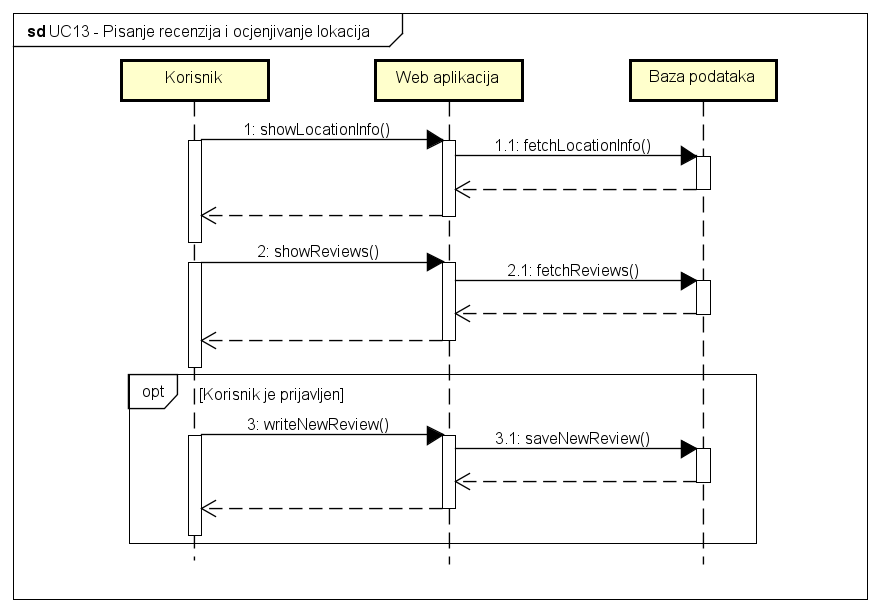
\includegraphics[width=\textwidth]{img/UC13-Pisanje_recenzija_i_ocjenjivanje_lokacija.png}
				\caption{Sekvencijski dijagram pisanja recenzija i ocjenjivanja lokacija}
			\end{figure}
    
    \pagebreak \section{Ostali zahtjevi}
	\begin{itemize}
		\item Dohvaćanje podataka iz baze podataka ne smije trajati dulje od nekoliko sekundi
		\item Lozinke i ostali povjerljivi podaci u bazi podataka moraju biti kriptirani
		\item Neispravno korištenje korisničkog sučelja i neispravan unos podataka ne smiju narušiti funkcionalnost aplikacije i integritet baze podataka
		\item Sustav treba biti implementiran kao web aplikacija koristeći objektno-orijentirane jezike
		\item Sustav treba funkcionirati pri istovremenom korištenju više korisnika
		\item Korisničko sučelje treba biti jednostavno i intuitivno za korištenje
		\item Nadogradnje sustava ne smiju narušavati postojeće funkcionalnosti sustava
		\item Veza s bazom podataka mora biti kvalitetno zaštićena, brza i otporna na vanjske greške
		\item Pristup sustavu mora biti omogućen iz javne mreže pomoću HTTPS
	\end{itemize}